\documentclass[12pt]{article}
\usepackage[a4paper, top=16mm, text={170mm, 248mm}, includehead, includefoot, hmarginratio=1:1, heightrounded]{geometry}
\usepackage{amsmath,amssymb,mathrsfs,amsthm,tikz,shuffle}
\usepackage{dsfont}
\usepackage{color}
\usepackage{ccfonts}
\usepackage[T1]{fontenc}
\renewcommand{\baselinestretch}{1.1}

\theoremstyle{definition}
	\newtheorem{para}{}[section]
		\renewcommand{\thepara}{\thesection.\arabic{para}}
	\newtheorem{exa}[para]{Example}
\theoremstyle{plain}
	\newtheorem{lem}[para]{Lemma}
	\newtheorem{thm}[para]{Theorem}
	\newtheorem{pro}[para]{Proposition}
\renewcommand{\proofname}{Proof}


%+++++++++++++++++++++++数学字体的设置++++++++++++++++++++++++++++++++++++++++%
\newcommand{\me}{\mathrm{e}}  % for math e
\newcommand{\mi}{\mathrm{i}} % for math i
\newcommand{\dif}{\mathrm{d}} %for differential operator d
\newcommand{\cvec}[1]{\!\vec{\,#1}}
\newcommand{\Ptimes}{\,\overset{\otimes }{,}\,}
\DeclareSymbolFont{lettersA}{U}{txmia}{m}{it}
 \DeclareMathSymbol{\piup}{\mathord}{lettersA}{25}
 \DeclareMathSymbol{\muup}{\mathord}{lettersA}{22}
 \DeclareMathSymbol{\deltaup}{\mathord}{lettersA}{14}
 \newcommand{\uppi}{\piup}

\pagestyle{plain}
\definecolor{shadecolor}{RGB}{32,32,32}
%\definecolor{textcolor}{RGB}{204,204,255}
%\definecolor{textcolor}{RGB}{224,224,224}
\definecolor{textcolor}{RGB}{204,255,204}
%\pagecolor{shadecolor}
%\color{textcolor}

\begin{document}

\section{Introduction}

Very recently, a vast generalization of tree level strings integrals has been proposed in \cite{}. This generalization is realized by identifying the Parke-Taylor form 
\[
	\mathsf{PT}(n):=\frac{\dif^{n}z}{\mathrm{SL}(2,\mathds{R})} \prod_{i=1}^{n}\frac{1}{z_{i}-z_{i+1}}
\]
as the canonical form of the moduli space $\mathcal{M}_{0,n}^{+}$ and the Koba-Nielson factor as a regulator of the divergent integral $\int \mathsf{PT}(n)$. With a positive parameterization  $\mathbf{x}:= \{x_{1},\cdots, x_{n-3}\}$  of $\mathcal{M}_{0,n}^{+}$, $\mathsf{PT}(n)$ becomes the canonical form $\prod_{i=1}^{n-3} \dif \log x_{i}$ of $\mathds{R}_{+}^{n-3}$ and the Koba-Nielson factor $\prod_{i<j} (z_{i}-z_{j})^{s_{ij}}$ becomes a product of powers of some Laurent polynomials $p_{I}(\mathbf{x})$, then string integrals end up with the form of
\begin{equation} 
	\int_{\mathds{R}_{+}^{D}} \prod_{i=1}^{D}\frac{\dif x_{i}}{x_{i}}x_{i}^{\alpha' X_{i}}\prod_{I}p_{I}(\mathbf{x})^{-\alpha'c_{I}}	\:, \label{int1}
\end{equation}
where $D=n{-}3$, $X_{i}$ and $c_{I}$ are linear combinations of Mandelstam variables $s_{ij}$'s. A \emph{stringy} integral is a integral of form eq.(\ref{int1}) but with arbitrary substraction-free polynoimals $p_{I}$. 

% In string theory, the tree level $n$-pt open superstring amplitudes
% \[
% 	I=\int_{\mathcal M_{0,n}^+}\frac{\dif^{n}z/\operatorname{SL}(2,\mathbb C)}{(z_1-z_2)\cdots (z_n-z_1)}\prod_{i<j}
% 	|z_i-z_j|^{\alpha' s_{ab}}
% \]
% is defined on a component $\mathcal M_{0,n}^+$ defined by $z_1<z_2<\cdots < z_n$ 
% of real points of moduli space of $n$ punctures on the Riemann sphere. 
% In the language of positive geometry \cite{}, $\mathcal M_{0,n}^+$ is a positive
% geometry and $\frac{\dif^{n-3}z}{(z_1-z_2)\cdots (z_n-z_1)}$ is its canonical form. Therefore,
% we can consider the generalized integral 
% \[
% 	I(\alpha')=\int_{x\in \mathcal P} \Omega_{\mathcal P} F(x)^{-\alpha'},
% \] 
% where $\mathcal P$ is a positive geometry, $\Omega_{\mathcal P}$ is its canonical form
% and $F(x)$ is a function defined on $\mathcal P$. In order to make $I(\alpha')$ a 
% well-behaved function of $\alpha'$, we usually further require that $F(x)$ has no pole
% and zero in the interior of $\mathcal P$. 

% In this article, we will not consider the so general integral above, we only consider the 
% following integrals, that is called stringy integrals, 
% \begin{equation}\label{int1}
% 	I(\mathbf X,\{c_I\}):=\int_{\mathbb R_+^D}\prod_{i=1}^D\frac{\dif x_i}{x_i}x_i^{\alpha' X_i}
% 	\prod_{I} p_I^{-\alpha' c_I}
% %	\quad\text{or}\quad
% %	\int_{[0,1]^D}\prod_{i=1}^D\frac{\dif x_i}{x_i(1-x_i)}\prod_{I} q_I^{-\alpha' c_I},
% \end{equation}
% where $p_a$ are all Laurent polynomial of $x$ with non-nagetive coefficients. 
% %These two integral can be related by the change of variables $x_i\mapsto x_i/(1+x_i)$.
% In fact, a wide class of general integrals 
% will turn into this form after finding a positive parameterization. 

In \cite{}, many important properties of stringy integrals are well studied, especially the relation between their field theory limit, {\it{i.e}}. the limit of $\alpha'\to 0$, and the Minkowski sum $N_{P}$ of Newton polytopes of $\{p_I\}$.
%As in the original superstring amplitude, the field theory limit of a stringy integral is  its leading order as $\alpha'\to 0$. 
More concretely, {\it{ i) the leading order of a stringy integral is given by the volume of the dual polytope, or the canonical function $\underline{\Omega}(N_{P})$, of $N_{P}$, and ii) a bijection between $\mathds{R}_{+}^{n-3}$ and $N_{P}$ is given by the siddle point equation of the regulator, that is the so-called scattering-equation map $\Phi$,}}
\begin{equation} \label{SEmap}
	X_{i}= \sum_{I}c_{I}\frac{\partial \log p_{I}}{\partial \log x_{i}}\:, \qquad  \text{for }i=1,\cdots,n{-}3.
\end{equation}	
In general, however, it's difficult to calculate the leading order of stringy integrals directly from the above two properties.
On the one hand, performing Minkowski sum for polytopes analyticly is nearly impossible. On the other hand, to obtain the canonical form $\Omega(N_{P})$ from the pushforward $\Phi_{\ast}\bigl(\bigwedge_{i=1}^{D} \dif \log x_{i}\bigr)$ requires to solve highly non-linear equations, just like the case in CHY formalism.


The main purpose of this article is to show an efficient method, {\it{blowing up}} (\textcolor{red}{C: or blowing-up map?}), to calculate the leading order of the integral eq.\eqref{int1} with respect to $\alpha'$. This is a general method which also is closely related to the {\it sector decomposition} prescription \cite{} used in Feynman integrals. We will see that the situation is easier when this method is applied in stringy integrals due to some features of canonical forms (\textcolor{red}{C: Is this sentence proper?\& How to introduce the proof about scattering-equation map?}).

(\textcolor{red}{C: Cohesiveness is needed.})
%give a direct proof of the second property, first given in \cite{}. 
%Finally, we give some examples and applications of these two method.
%Let's make a glance what we have done in this article.

%Consider a vertex $V$ of $\mathcal P$, locally it's defined by $x_1=\cdots = x_D=0$ so that 
%near the vertex, the integral reads

% For the first part, we first note that when $\alpha'\to 0$, the pole structure of 
% canonical form leads that the contribution of the integral near a codimension $k$ face
% diverges as $(\alpha')^{-k}$, so the leading terms come from vertices.

It is obvious that the leading order contribution in $\alpha'$-expansion of stringy integrals arise from each vertex of the integration reigon $\mathds{R}_{+}^{D}$. Since every vertex can be brought to the origin by replacing $x_{i}$ with $x_{i}^{-1}$, it is sufficient to work out the contribution from the origin only. Now, suppose that all $p_I(0)\neq 0$ in the integral eq.\eqref{int1}, then the integral at the neighbourhood of the origin becomes 
\begin{equation}\label{int2}
	\int_{[0,\epsilon]^D}\prod_{i=1}^D\frac{\dif x_i}{x_i}x_i^{\alpha' X_i} \prod_{I}p_{I}(0)^{-\alpha' c_{I}}
	=\prod_{i=1}^D\frac{\epsilon^{\alpha' X_i}p_{I}(0)^{-\alpha' c_{I}}}{\alpha' X_i}
	\sim \frac{1}{(\alpha')^D}\frac{1}{X_1\cdots X_D}+O(\alpha'^{-D+1}).
\end{equation}
%Geometrically, it's so simple because it's only $x_1=\cdots=x_D=0$ that defines the vertices. 
Generally, it would not be such simple case, there woule be two obstacles
\begin{itemize}
	\item Some polynomials $p_I$ may vanish at the origin (or a vertex).
	\item Furthermore, some $p_I$ may own the origin (or a vertex) as their singular point\footnote{A point $Q$ is a singular point of the surface defined by $p(\mathrm{x})$=0 if $p(Q)=0$ and $\partial p(Q)/\partial x_{i} =0$ for all $i$}.
\end{itemize}
They can be overcome by a series of blowing up. After these blow-ups, the 
stringy integral is decomposed into many integrals like eq.\eqref{int2}, then the leading order is given by summation.

In the second part, we give a direct proof of a proposition firstly given in \cite{} that 
the scattering-equation map \eqref{SEmap} from the saddle point equations of the integral eq.\eqref{int1} 
is a one-to-one map from the interior of $\mathbb R_+^D$ to the interior of Minkowski sum of 
Newton polytopes of $p_I$. ...

Finally, ...

\section{Blow up}

% \begin{figure}[t]
% \begin{center}
% 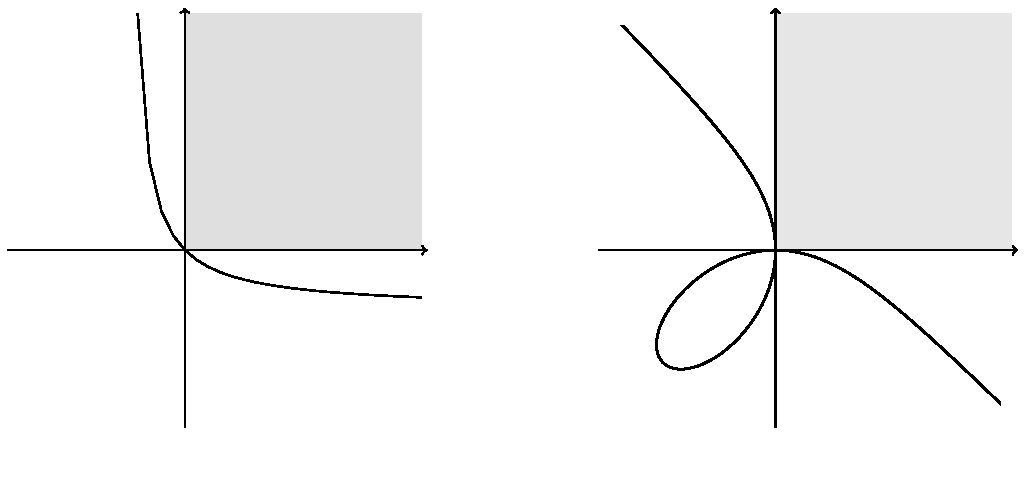
\includegraphics[scale=0.75]{fig_1.pdf}
% \end{center}
% \vspace{-5ex}
% \caption{Left: $p=x+y+xy$, Right: $p=x^3+y^3+xy$}
% \end{figure}

(Some review of positive geometry \& canonical form. ...)

As mentioned in the introduction, leading order of the integral eq.\eqref{int1} comes from the vertex
of the integral region. 
At each vertex, generally there're two main difficulties to work out the leading terms
\begin{itemize}
	\item There're some polynomials $p_I$ other than $x_i$ vanishing at a vertex.
	\item Furthermore, the vertex is usually a singularity of $p_I$.
\end{itemize}
For example, for the integral 
\[
	\int_0^\infty \int_0^\infty \frac{\dif x}{x}\frac{\dif y}{y}x^{\alpha' X}
	y^{\alpha' Y}(x+y+ xy)^{-\alpha' c},
\] 
the vertex $(0,0)$ is the common zero set of three polynomials $x$, $y$ and $x+y+xy$. 
Further, for the integral 
\[
	\int_0^\infty \int_0^\infty \frac{\dif x}{x}\frac{\dif y}{y}x^{\alpha' X}
	y^{\alpha' Y}(x^3+y^3+ xy)^{-\alpha' c},
\] 
the vertex $(0,0)$ is a singularity of the curve $x^3+y^3+xy=0$. 

% In the blowing up, the above two example becomes 
% \[
% 	p=t(u+v+tuv) \quad\text{and}\quad p=t^2(tu^3+tv^3+uv)
% \]
% respectively.

%Consider the integration
%\begin{equation}\label{int}
%	I(\alpha')=\int_{\mathcal P} \Omega_{\mathcal P}(x)\prod_i(p_i(x))^{\alpha' s_i},
%\end{equation}
%where $\Omega$ is the canonical form of the $D$-dimensional positive geometry $\mathcal P$, and we suppose $I(\alpha')$ is finite when $\alpha'>0$.
%It's clear that $I(\alpha')$ diverge when $\alpha'\to 0$ because the simple pole of canonical form on the boundary of $\mathcal P$. We want to calculate the leading order of its Laurent series with respect to $\alpha'$ at $\alpha'=0$. % It's a rational function of $s_i$ since $p_i$ are all polynomials.
%
% Consider the following integral
% \[
% 	\int_{\mathbb R_+^d}\frac{d x_1}{x_1} \cdots \frac{d x_d}{x_d} x_1^{n_1}\cdots x_d^{\alpha' n_d} P(x_1,\dots,x_d)^{-\alpha' c}, 
% \]
% where $P$ is a polynomial, here we can further assume that $P(0,\dots,0)\neq 0$. When $\alpha'\to 0$, the integral diverge, we want to calculate the leading term of $(\alpha')^{-1}$ of this integral. blabla

% Let's first consider the one-dimensional example, the Beta function 
% \[
% 	B(\alpha' a,\alpha' b)=\int_0^1 \frac{dt}{t(1-t)}\, t^{\alpha' a}(1-t)^{\alpha' b}.
% \]
% To calculate the integral, we can decompose the integral by 
% \[
% 	\biggl(\int_{0}^\epsilon +\int_\epsilon^{1-\epsilon}+\int_{1-\epsilon}^1\biggr) \frac{dt}{t(1-t)}\, t^{\alpha' a}(1-t)^{\alpha' b}.
% \]
% The middle integral is finite when $\alpha'\to 0$ so that it does not contribute, the other two integrals are
% \[
% 	\int_0^\epsilon  \frac{dt}{t(1-t)}\, t^{\alpha' a}(1-t)^{\alpha' b}
% 	\sim \int_0^\epsilon \frac{dt}t t^{\alpha' a} 
% 	= \frac{\epsilon^{\alpha' a}}{\alpha'a} \sim \frac{1}{\alpha'a},
% 	\]
% \[
% 	\int_{1-\epsilon}^1  \frac{dt}{t(1-t)}\, t^{\alpha' a}(1-t)^{\alpha' b}
% 	\sim \int_0^\epsilon \frac{dt}{t}\, t^{\alpha' b} \sim \frac{1}{\alpha' b},
% \]
% so the leading term of this integral is 
% \[
% 	B(\alpha' a,\alpha' b)\sim\frac 1{\alpha'}\biggl(\frac 1a+\frac 1b\biggr).
% \]
% 
% One important lesson from the above trivial integral is that the leading terms of the integral come from the vertices of the positive geometry. 

Let's give a short review of blow up. 
One main purpose of blowing-up in math is to resolve singularities. 
Let's first consider a simple example. 
Suppose there's a family of line $\{l_i: a_ix+b_iy=0\}_{i=1,\dots,n}$ crossing 
the original point. The point $(0,0)$ is the common zero set of these lines,
however it only contains little information of these lines. In another viewpoint,
$(0,0)$ is a `singularity' because generally $n$ lines cannot cross each other 
at a common point on the plane. 

If one wants know the information of these lines even when $(x,y)\to (0,0)$, 
or equivalently to resolve the singularity at $(0,0)$, one can introduce the 
change of variabes:
\[
	x=ut,\quad y=vt,
\] 
where $[u,v]$ is a projective coordinate, otherwise any common factor of $u$ and $v$ can be 
absorbed into the definition of $t$, so that line equations become 
\[
	a_i u + b_i v = 0,
\]
and the solution is $[u,v]=[-b_i,a_i]$. In terms of old variables, every information 
becomes a point $(0,0)$ in $\mathbb R^2$, but in new variables or in space 
$\mathbb R\times \mathbb P^1$, lines become $(0,[-b_i,a_i])$ so that 
we can read the imformation even $(x,y)=(0,0)$. 
The idea described here is called blowing-up in math.  
The above example is called the blowing-up of the plane along the original point, which 
resolves the singularity at $(0,0)$. We will consider the blowing-up of $\mathbb R^D$
along subspace $\mathbb R^n$ defined by $x_{i_1}=\cdots=x_{i_n}=0$. 
The blow-up is the surface defined by $x_{i_j}y_k=x_{i_k}y_j$ in space 
$\mathbb R^{N}\times \mathbb P^{n-1}$,
where $[y_1,\dots,y_n]$ is the projective coordinate. These equation can be easily
solved by $y_j=tx_{i_j}$ for $t\neq 0$.
%Generally, let $X=\operatorname{Spec} A$ be an affine scheme, and let $V(f_1,\dots,f_n)\subset X$
%is a closed subscheme of $X$. The blow-up of $Y$ in X is the closure in
%$X\times_A \mathbb P_A^{n-1}=\mathbb P_A^{n-1}$ of the graph of the morphism 
%\[
%\alpha_{(f_1,\dots,f_n)}:X-Y\to \mathbb P_A^{n-1}.
%\] 

% Generally,
% general blowing up must have the form of $x_i=ty_i$ locally althought it may be very difficult
% to construct a blowing-up globally.

Now let's carefully consider the first example,
\[
	I=\int_0^\infty \int_0^\infty\frac{dx}{x}\frac{dy}{y}x^{\alpha' a}y^{\alpha' b}(x+y+x y)^{-\alpha' c}.
\]
The leading terms come form the neighbourhoods of four vertices $(0,0)$, $(0,\infty)$, $(\infty,0)$ and $(\infty,\infty)$. Let's consider the simplest vertex first, 
\[
	I(0,\infty)=\int_{0}^\epsilon\int_{1/\epsilon}^\infty \frac{dx}{x}\frac{dy}{y}x^{\alpha' a}y^{\alpha' b}(x+y+xy)^{-\alpha' c}\sim \int_{0}^\epsilon\int_{1/\epsilon}^\infty \frac{dx}{x}\frac{dy}{y}x^{\alpha' a}y^{\alpha' (b-c)}\sim 
	\frac{1}{{\alpha'}^2}\frac{1}{a} \frac{1}{c-b}
\]
Near the vertex $(0,\infty)$, the integral decouples because the mixed factor $x+y+xy \sim y$ when $y \gg x$.  Similarly, $I(\infty,0)\sim ({\alpha'}^2 b (c-a))^{-1}$. 

For the harder vertex
\[
I(0,0)=\int^{\epsilon}_0 \int^{\epsilon}_0 \frac{dx}{x}\frac{dy}{y}x^{\alpha' a}y^{\alpha' b}(x+y+xy)^{-\alpha' c}
%\sim\int^{\epsilon}_0 \int^{\epsilon}_0\frac{dx}{x}\frac{dy}{y}x^{\alpha' a}y^{\alpha' b}(x+y)^{-\alpha' c}.
\]
when $(x,y)\to (0,0)$, we cannot decouple $x$ and $y$ in the mixed factor $(x+y+xy)^{-\alpha' c}$ 
because we don't know which one is dominated. However, we can drop the term $xy$ because $xy\ll x$, $y$. 
For the remaining terms $x+y$, we can introduce new variables $x = tp$ and $y=t(1-p)$, then
\begin{equation}\label{canonicalformunderblowup}
	\frac{dxdy}{xy} = \frac{dp}{p(1-p)}\frac{dt}{t},
\end{equation}
and
\begin{equation*}
	i(0,0)=\int_{1/\epsilon}^\infty\frac{dt}{t} t^{\alpha'(a+b-c)}\int_0^{1}\frac{dp}{p(1-p)}p^{\alpha' a}(1-p)^{\alpha' b}%\sim \frac{1}{\alpha'}\frac{1}{a+b-c}\int_0^{1}\frac{dp}{p(1-p)}p^{\alpha' a}(1-p)^{\alpha' b}
	\sim \frac{1}{{\alpha'}^2}\frac{1}{c-a-b}\biggl(\frac 1a+\frac 1b\biggr).
\end{equation*}
in this example, whether $x$ or $y$ is dominated in the integration is characterized by $p$, 
and both vertices $p\sim 0$ ($x\ll y$) and $p\sim 1$ ($y\ll x$) contribute.
\begin{center}
\begin{tikzpicture}[scale=0.8]
\fill[gray!30,opacity=0.4] (-6.9,1.4) -- (-3.9,1.4) -- (-3.9,4.4) -- (-6.9,4.4);
\draw[->] (-7,1.4) -- (-3.9,1.4);
\draw[->] (-6.9,1.3) -- (-6.9,4.4);
\draw[densely dotted]  (-6.9,1.4) ellipse (0.5 and 0.5);
\draw[->] (-6.9,1.2) .. controls (-6.9,0.4) and (-6.7,0) .. (-4.7,0);
\fill[gray!30,opacity=0.4] (-3.5,-0.8) -- (-1.5,-0.8) -- (-1.5,2.2) -- (-4.5,2.2) -- (-4.5,0.2);
\draw[->] (-4.6,-0.8) -- (-1.5,-0.8);
\draw[->] (-4.5,-0.9) -- (-4.5,2.2);
\draw (-3.5,-0.8) -- (-4.5,0.2);
\draw[densely dashed,->] (-4.5,0.2) -- (-3.2,-1.1)node[right]{$p$};
\draw[->]  plot[smooth, tension=.7] coordinates {(-4.4,0.3) (-2.7,1.7) (-0.6,2)};
\draw[->]  plot[smooth, tension=.7] coordinates {(-3.5,-0.9) (-2.4,-2.4) (-0.6,-2.6)};
\fill[gray!30,opacity=0.4] (0.8,-3.4) -- (2.8,-3.4) -- (2.8,-0.4) -- (-0.2,-0.4) -- (-0.2,-3.4);
\draw[->] (-0.3,-3.4) -- (2.8,-3.4);
\draw[->] (-0.2,-3.5) -- (-0.2,-0.4);
\fill[gray!30,opacity=0.4] (0.8,1) -- (2.8,1) -- (2.8,4) -- (-0.2,4) -- (-0.2,1);
\draw[->] (-0.3,1) -- (2.8,1);
\draw[->] (-0.2,0.9) -- (-0.2,4);
\node at (-2.8,2) {\small $p\sim 0$};
\node at (-2.2,-2) {\small $p\sim 1$};
\node at (-4,-1) {\small $t$};
\node at (-4.6,-0.4) {\small $t$};
\node at (2.8,0.8) {\small $p$};
\node at (-0.4,4) {\small $t$};
\node at (-0.4,-0.4) {\small $t$};
\node at (2.8,-3.6) {\small $1-p$};
\end{tikzpicture}
\end{center}
Similarly, one can work out $I(\infty,\infty)$, and the finally
\[
	I\sim I(0,0)+I(0,\infty)+I(\infty,0)+I(\infty,\infty).
\] 
%similarly, 
%\[
%	I(\infty,\infty)\sim \frac{1}{{\alpha'}^2}\frac{1}{c-a-b}\biggl(\frac 1{c-a}+\frac 1{c-b}\biggr),
%\]
%so the leading terms of original integral is 
%\[
%	I\sim I(0,0)+I(0,\infty)+I(\infty,0)+I(\infty,\infty).
%\]

Now for the second example, near $(0,0)$, blow up $p=x^3+y^3+x y$ by letting
$x=tu$ and $y=tv$, then when $u\sim 1$, 
$p=t^2(t +t v^3+ v)\sim t^2(t+v)=t(x^2+y)$. 
Similarly, if $v=1$, we will get $p\sim t(x+y^2)$. 
If we draw new curves $x^2+y=0$ and $x+y^2=0$ and the old curve $x^3+y^3+xy$, 
we can see that the original curve
decomposes into two curves generated by blowing up in the above diagram, so that 
the contribution of integral is also decomposed.
% \begin{center}
% 	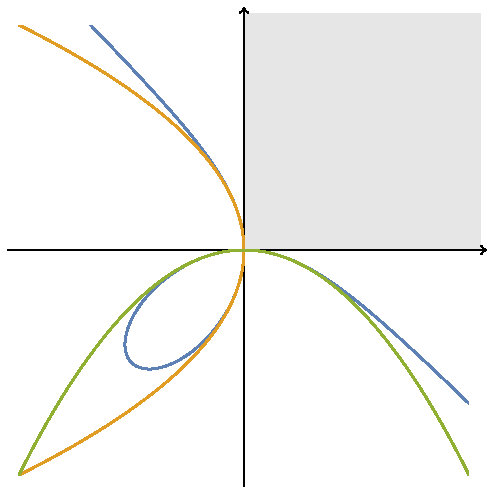
\includegraphics[scale=0.7]{fig_2.pdf}	
% \end{center}
where the blue curve is $x^3+y^3+xy=0$, the green curve is $y+x^2=0$ and
the orange curve $x+y^2=0$.

In other words, in the expansion 
\[
	(y+x^2)(x+y^2)=xy+x^3+y^3+xy^2+x^2y+x^2y^2\sim x^3+y^3+xy,
\]
$xy^2$, $x^2y$, $x^2y^2\ll xy$ so that they don't contribute in the integral near $(0,0)$.
Next we will carefully consider which terms we can throw away.

% Generally, we want to decompose a polynomial into
% \[
% 	p\sim \prod_{i\leq j} \prod_k (x_i^{a^k_{ij}}+x_j^{b^k_{ij}})
% \]

Now let's consider the general story. Generally, the integral near a vertex need not to be decoupled as $I(0,\infty)$ above, so blowing-up is necessary. Suppose we come to the vertex defined locally by $x_1=\cdots=x_D=0$, 
\[
	I(0,\dots,0)\sim \int_{[0,\epsilon]^D} \frac{d x_1}{x_1}\cdots \frac{d x_D}{x_D} \prod_i(p_i(x))^{\alpha' s_i}.
\]
In each polynomial $p_i$, 
\[
	p_i(x)=\sum_{I} a_{iI} x^{n^I},
\]
we need to worry about which $x^{n^I}$ is dominated in the integration, however not all terms can dominate 
the integral. For example, if we find that $x^{n^J}=x^{n^I}x^{v}$ or equivalently $n^J=n^I+v$ for some 
non-zero positive vector $v$, there's no need to consider $x^{n^J}$ anymore because it goes to zero faster 
than $x^{n^I}$. Geometrically, one can assign each term with a cone $C_{I}=(n^I+\mathbb R^D_{+})$, the above
claim is equivalently that other terms in this cone can be throw away.

Furthermore, we can consider the convex hull of these cones $\{C_I\}$. It's usually larger than
the union of these cones $\bigcup_I C_I$, but terms other than vertices in $C$ are also not dominated!
Here let's consider an example $p(x)=x^6+y^6+x^2y^2$. 
\begin{center}
	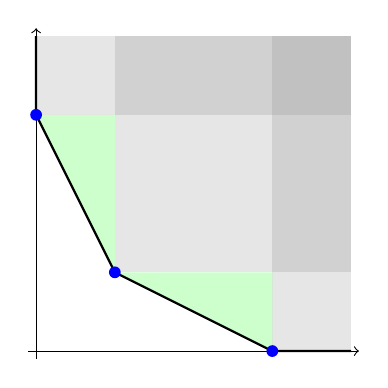
\begin{tikzpicture}
		\fill[gray,opacity=0.2] (0,4) -- (0,3) -- (4,3) -- (4,4);
		\fill[gray,opacity=0.2] (1,4) -- (1,1) -- (4,1) -- (4,4);
		\fill[gray,opacity=0.2] (3,4) -- (3,0) -- (4,0) -- (4,4); 
		\fill[green,opacity=0.2] (0,3) -- (1,3) -- (1,1); 
		\fill[green,opacity=0.2] (3,0) -- (3,1) -- (1,1); 
		\draw[thick] (0,4) -- (0,3) -- (1,1) -- (3,0) -- (4,0);
		\draw[->](-0.1,0) -- (4.1,0);
		\draw[->](0,-0.1) -- (0,4.1);
		\node[inner sep=1.5pt,circle,fill=blue] at (0,3) {};
		\node[inner sep=1.5pt,circle,fill=blue] at (1,1) {};
		\node[inner sep=1.5pt,circle,fill=blue] at (3,0) {};
	\end{tikzpicture}
\end{center}
In the above diagram, besides gray cones, the convex hull contains two green regions. 
If we add terms like $x^5y^2$ in the interior of green regions to the polynomial, 
we will show that the leading terms of the integral from this vertices $x_1=x_2=\cdots=x_D=0$
do not change.

\begin{lem}
Suppose $p$ is a polynomial $p(x)=\sum_{I\in \mathscr A}a_I x^{n^I}$, and $C[p]$ is the convex hull
of $\{C_{I}=(n^I+\mathbb R^D_{+})\}$. When we consider the integral near the vertices $x_1=\cdots=x_D=0$, 
then we can replace $p(x)$ by a new polynomial $\bar p(x)=\sum_{J\in \mathscr B}a_J x^{n^J}$ such that
the leading terms will not change.
\end{lem}

% In the following proof, we define $|v|=\sum_{i=1}^D v_i$ for any vector $v\in \mathbb R^D$.

\begin{proof}
We have seen that terms other than vertices in $\bigcup_I C_I$ do not contribute. Suppose a term $x^v$ 
is in the interior of $C[p]-\bigcup_I C_I$,  
then there exist non-negative numbers $\{c_J\}$ such that it can be written as 
\[
	v = \sum_{J\in \mathscr B}c_J n^J,\quad \sum_{J\in \mathscr B} c_J>1.
\]
If $x^{n^L}$ dominates some limit process, 
then for other $J\in \mathscr B$, there exists a non-negative number $r_J$ such that
$x^{w^J}:=x^{n^L-n^J}\leq r_J$, then 
\[
	x^v = \prod_{J\in\mathscr B} (x^{n_J})^{c_J} = 
	(x^{n_L})^{\sum_J c_J}\prod_{J\in \mathscr B} 
	(x^{w_J})^{c_J}\leq R\,(x^{n_L})^{\sum_J c_J}
\] 
where $R$ is a non-negative number and $\sum_J c_J>1$, so $x^v$ goes to 
zero faster than $x^{n_L}$. Since $L\in \mathscr B$ is arbitrary, $x^v$ can be throw away.

Finally, suppose that $v$ is on the boundary of $C[p]$ but it's not a vertex.
% then it can be written as 
% \[
% 	v = \sum_{J\in \mathscr C}c_J n^J,\quad \sum_{J\in \mathscr C} c_J=1,
% \]
% where $\mathscr C$ is the set of vertices on the same boundary as $v$.
We can prove the result by showing this terms goes to zero faster than some vertices on the 
same boundary, so we can further assume that $p$ is a homogeneous polynomial.
After blowing-up, near the new vertex
$y_i=1$, the polynomial becomes $p'=t^{\sum_i v_i}\sum_{I}a_I y^{n^I}|_{y_i=1}$. 
Since $v$ is not a vertex, it should be in the interior of the cone of this new polynomial or 
on the boundary of the cone (for all $i$), and then by 
the proven part of lemma and induction on codimension, it doesn't contribute the integral.
\end{proof}

In other words, we have proven the following proposition. 

\begin{pro}
The leading order of integrals
\[
	I=\int_{[0,\epsilon]^D} \left(\prod_{i=1}^D\frac{\dif x_i}{x_i}x_i^{\alpha' X_i}\right)
	p_1^{-\alpha' c} \prod_I q_I^{-\alpha' c_I}
	\quad \text{and} \quad 
	I'=\int_{[0,\epsilon]^D} \left(\prod_{i=1}^D\frac{\dif x_i}{x_i}x_i^{\alpha' X_i}\right)
	p_2^{-\alpha' c} \prod_I q_I^{-\alpha' c_I}
\]
are the same if and only if $C[p_1]=C[p_2]$.
\end{pro}

From the theorem in \cite{}, the leading order of the integral eq.\eqref{int1} 
only depands on the Minkowski sum of Newton polytopes of polynomials $p_I$, 
the above proposition is just like the local version of this theorem, so that 
it seems trivial. However, it's more free to use the local version because 
the cone is not as rigid as the Newton polytopem, and it just looks  
like a `corner' of the Newton polytope.

% Geometrically, if we consider the cone $C$ spanned by all $\{n^I\}$, then the basis can be choosen as the vertices on the boundary of $C$, and terms corresponding to points inside $C$ can be dropped.
% For example, suppose that $p(x,y)=x^3+y^3+xy+x^3y^2+xy^3$, we draw each $n^I$ in the following diagram,
% \begin{center}
% 	\begin{tikzpicture}
% 		\fill[gray!20] (0,4) -- (0,3) -- (1,1) -- (3,0) -- (4,0) -- (4,4);
% 		\draw[thick] (0,4) -- (0,3) -- (1,1) -- (3,0) -- (4,0);
% 		\draw[->](-0.1,0) -- (4,0);
% 		\draw[->](0,-0.1) -- (0,4);
% 		\node at (3,2) {$\times$};
% 		\node at (3,1.5) {$x^3y^2$};
% 		\node at (1,3) {$\times$};
% 		\node at (1,2.5) {$xy^2$};
% 		\node[inner sep=1.5pt,circle,fill=blue] at (0,3) {};
% 		\node[inner sep=1.5pt,circle,fill=blue] at (1,1) {};
% 		\node[inner sep=1.5pt,circle,fill=blue] at (3,0) {};
% 	\end{tikzpicture}
% \end{center}
% where $x^3y^2\leftrightarrow (3,2)$ and $xy^3\leftrightarrow (1,3)$ are represented by $\times$ in the diagram and other terms are represented by blue points. The basis is given by blue points $\{x^3\leftrightarrow (3,0),y^3\leftrightarrow (0,3),xy\leftrightarrow (1,1)\}$, and the gray region is the set of all vectors $v=\sum_{J\in \mathscr B}c^I_J n^J$ where $\sum_J c^I_J>1$, therefore we throw away terms in the gray region and then get that $\bar p(x)=x^3+y^3+xy$. 

Now, after drawing the cone of a polynomial $p$, if one get
\begin{center}
\begin{tikzpicture}[scale=0.75,baseline={([yshift=-.5ex]current bounding box.center)}]
\fill[gray!20] (2,3) -- (0,3) -- (0,0) -- (3,0) -- (3,1) -- (3,3);
\draw[->](-1.1,-0.5) -- (3,-0.5);
\draw[->](-1,-0.6) -- (-1,3);
\draw[->] (-1,-0.5) -- (0,0);
\node at (-0.5,0) {$v$};
\end{tikzpicture}
\end{center}
then we call that $p(x)\sim x^v$ is decoupled. 
In other words, $p$ has the form of 
\[
p(x)=x^v(c+q(x)),
\] 
where $q(0)=0$ and $v$ is a vector. 
Our next aim is to find a series of blow-ups to make all polynoimals 
decouple in this way.

Now we start to consider how to blow up. 
As has seen from eq.\eqref{canonicalformunderblowup}, one important feature of $\Omega_{\mathcal P}$
is `invariant' under the blowing-up because the residue of the canonical form on the boundary is
the canonical form of the boundary.

Suppose we blow up near the boundary defined locally by $x_1=\cdots=x_n=0$ in integral eq.\eqref{int1}. 
It's already the most general cases. In fact, if in the definition of a boundary $x_i=\infty$, we can
change the variable $x_i\mapsto 1/x_i$ and then $x_i=0$.
Let $x_i=ty_i$, where $[y_1,\dots,y_n]$ are positive projective coordinates. 
Near the boundary, the canonical form of $\Omega$ performs as 
\[
	\Omega=\frac{dx_1}{x_1}\wedge \cdots\wedge\frac{dx_n}{x_n}
	\wedge \Phi(x'),
\]
where $x'$ are other coordinates. In new coordinates, it can be written as 
\[
	\Omega=\frac{1}{y_n}\frac{dt}{t}\wedge \frac{dy_1}{y_1}\wedge \cdots
	\wedge\frac{dy_{n-1}}{y_{n-1}}\wedge \Phi(x')+O(t^0),
\]
where $y_n=1-(y_1+\cdots+y_{n-1})$ and $\Phi$ is the canonical form of the boundary of $\mathcal P$ given by $x_1=\cdots=x_n=0$. Therefore,
\[
	\operatorname{Res}_{t=0}(\Omega)=\frac{1}{y_n}\frac{dy_1}{y_1}\wedge \cdots\wedge\frac{dy_{n-1}}{y_{n-1}}\wedge \Phi(x')=\Omega_{n-1}(y)\wedge \Phi(x'),
\]
$\Omega_{n-1}(y)$ the canonical form of a standard $(n-1)$-dimensional simplex $\Delta_{n-1}$ defined by
$
	\sum_{i=1}^n y_i=1
$ and $y_i\geq 0$. 
% If we rewrite it in new coordinates $\{z_i\}$ such that
% \[
% 	z_0=0,\quad y_i=z_i-z_{i-1},\quad z_{n}=1,
% \]
% then 
% \[
% 	\Omega_{n-1}(z)=\frac{dz_1\wedge\cdots\wedge dz_n}{(z_1-z_0)\cdots (z_n-z_{n-1})}.
% \]
% It's the more familiar form.

% Consider a set of irreducible polynomials $\{p_i\}$, let $Z(p_i)$ be the zero point set of $p_i$ in $\mathbb{R}^n$. Suppose a curved polytope $\mathcal P$ is bounded by $\bigcup_i Z(p_i)$, if $F_k$ is a codimension $k$ face of $\mathcal P$ where $\#\{i\,:\,F_k\subset Z(p_i)\}>k$, then we call it a degenerated face.

% Now Consider the integration
% \[
% 	I(\alpha')=\int_{\mathcal P} \Omega_{\mathcal P}(x)\prod_i(p_i(x))^{\alpha' s_i},
% \]
% where $\Omega$ is the canonical form of $\mathcal P$, and we suppose $I(\alpha')$ is finite when $\alpha'>0$.
% It's clear that $I(\alpha')$ diverge when $\alpha'\to 0$. We want to find all possible poles in the leading order of its Laurent series with respect to $\alpha$ at $\alpha=0$. It's a rational function of $s_i$ since $p_i$ are all polynomials.

% If $F$ is a facet of $\mathcal P$. Locally, if $F$ is defined by $x=0$, then near $F$, the integration is 
% \[
% 	\int_0^\epsilon \frac{d x}{x} x^{\alpha' a} \int_{x'}\Psi(x')
% 	\sim \frac{1}{\alpha' a}\int_{x'}\Psi(x'),
% \]
% where $x'$ are other coordinates and $\Psi(x')$ is the left part of $\Omega_{\mathcal P}(x)\prod_i(p_i(x))^{\alpha' s_i}$.

For polynomials, suppose that 
$p_I(x) = t^{k_I}q_I(x',y,t)$.
Then the integral eq.\eqref{int1}, near this boundary and when $\alpha'$ is small, becomes
\[
\begin{aligned}
\int_{x'} \int_{x\in [0,\epsilon]^n} \Omega(x,x')\,\prod_ix_i^{\alpha' X_i}&
\prod_I(p_I(x))^{-\alpha' c_I}=
\int_0^\epsilon \, \frac{dt}{t} t^{\alpha'\sum_{i=1}^n X_i-\alpha' \sum_I k_Is_I}\\
	  &\int_{y\in\Delta_{n-1}}\Omega_{n-1}(y)
\prod_{j=1}^n y_j^{\alpha' X_j}
\int_{x'}\Phi(x')\prod_{k=n+1}^D(x'_k)^{\alpha' X_k}
\prod_I(q_I(x',y,t))^{-\alpha' c_I},
\end{aligned}
\]
however we still need to worry about the blowing-up of $t$, $y$ and $x'$ in $q_I$ because
it's still unknown that which one is dominated.

Blowing up produces new vertices 
$
	\{v_i:x'=0,t=0,y_i=1\}
$.
Note that $y_i=1$ means that $y_j=0$ for $j\neq i$ because $\sum_i y_i=1$. Therefore, it's equivalent to 
do such change of variables
\[
	x'\to x',\quad x_j\to tx_j\quad \text{for $j\neq i$},\quad x_i\to t,
\]
or just reuse the name of $x_i$ for $t$ to save the namespace,
\[
	x'\to x',\quad x_j\to x_ix_j\quad \text{for $j\neq i$},\quad x_i\to x_i,
\]
% which is related to the sector decompostion. 
% We will use this change of variable from now on.
In this change of variables, the polynomial $p=\sum_I a_I x^{n^I}$ becomes $p'=\sum_I a_I x^{(n^I)'}$, where
\[
	(n^I)'_i\longrightarrow \sum_j n^I_j,
\]
which can be visualized by the cone.
For example, for $p(x)=x^3+xy+y^3$, the gray cone, we first get the green cone, 
but it's not the wanted (decoupled) cone, so we blow up it again and we get the red cone.
\begin{center}
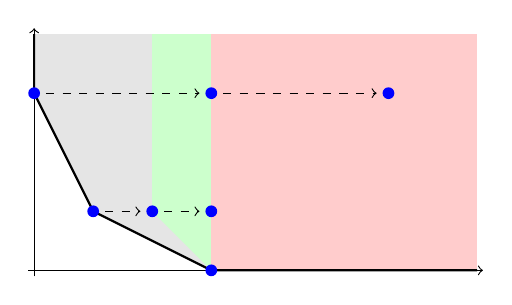
\begin{tikzpicture}[scale=0.75]
	\fill[gray!20] (0,4) -- (0,3) -- (1,1) -- (3,0) -- (4,0) -- (7.5,4);
	\fill[green!20] (2,4) -- (2,1) -- (3,0) -- (4,0) -- (7.5,4) --cycle;
	\fill[red!20] (3,4) -- (7.5,4) -- (7.5,0) -- (3,0)-- cycle;
	\draw[thick] (0,4) -- (0,3) -- (1,1) -- (3,0) -- (7.5,0);
	\draw[->](-0.1,0) -- (7.6,0);
	\draw[->](0,-0.1) -- (0,4.1);
	\node[inner sep=1.5pt,circle,fill=blue] at (0,3) {};
	\node[inner sep=1.5pt,circle,fill=blue] at (1,1) {};
	\node[inner sep=1.5pt,circle,fill=blue] at (3,0) {};
	\node[inner sep=1.5pt,circle,fill=blue] at (2,1) {};
	\node[inner sep=1.5pt,circle,fill=blue] at (3,3) {};
	\node[inner sep=1.5pt,circle,fill=blue] at (3,1) {};
	\node[inner sep=1.5pt,circle,fill=blue] at (6,3) {};
	\draw[dashed,->] (0.2,3) -- (2.8,3);
	\draw[dashed,->] (1.2,1) -- (1.8,1);
	\draw[dashed,->] (3.2,3) -- (5.8,3);
	\draw[dashed,->] (2.2,1) -- (2.8,1);
\end{tikzpicture}
\end{center}
Note that we still need to work out other vertices generated by blowing-up. 

Now, a natrual question arises. For a given polynomial $p$, 
can we terminate after finte steps such that near each generated vertex, $p$ becomes 
decoupled? This question is first declared by Hironake. He designed a game, which is 
called Hironaka's Polyhedra Game. Let's recall the game rule in our language.

Suppose $p$ is a given polynomial. There're two players A and B in the game. 
At each turn, first A choose a set of variables $\{x_{i_1},\dots,x_{i_n}\}$, then
B choose one variable $x_{i_k}$ out of them and make the change of variables 
$x_{i_j} \to x_{i_k}x_{i_j}$ for $j\neq k$.
If $p$ becomes decoupled, then A wins, otherwise they start a new turn by using the 
new generated polynomial. If A cannot win in finite steps, B wins.




% **Answer: Yes! [Hironake 67] However, sequences of blowing-up of a given polynomial
% need not to be unique.

% **The possible method: [Spivakovsky 83], [Encinas \& Hauser 02], [Zeillinger 05], \dots

However they are not so efficient. In our computation, we choose the minimal set of
variables such that $p=0$ after setting these variables to be zero. Usually, it's more 
efficient than the above methods, but it's not clear whether it can terminate. If not,
we can use any above method.

\section{Map}

Newton Polytope: For a substraction free Laurent polynomial 
\[
	f = \sum_{I\in \mathscr A} a_I \prod_{i=1}^n x_i^{n^I_i},
\]
we define the Newton polytope of $f$ by
\[
	N(f)=\operatorname{ConvexHull}\bigl(\{\mathbf n^I\,:\, I\in \mathscr A\}\bigr),
\]
where $\mathbf n^I=(n^I_1,\dots,n^I_n)$. The convex hull of vectors is defined
\[
	\operatorname{ConvexHull}\bigl(\{\mathbf n^I\,:\, I\in \mathscr A\}\bigr)
	=\Biggl\{\sum_{I\in\mathscr A}\lambda_I \mathbf n^I\,:\,
	\text{$\lambda_I>0$ and $\sum_I\lambda_I=1$}\Biggr\}.
\] 

Mink. Sum: Minkowski sum of two subsets $A$ and $B$ of $\mathbb R^n$ is defined by 
\[
	A+B=\{x+y\,:\,x\in A,\, y\in B\}.
\] 

(Some examples?)

...

In this section we present a proof to the statement:
\begin{pro}
For an arbitrary product of M polynomials $P=\prod_{j=1}^M p_j^{\alpha_j}$, $p_j=\sum_{I_j} a_{I_j} x^{I_j}$ with $a_{I_j}\geq 0$ for all $I_j$ and
 \[
	x^{I_j}:=\prod_{i=1}^D x_i^{n^{I_j}_i},
\]
whose Newton polytope is defined as the Minkowski sum  $N_P=\sum_j \alpha_j N(p_j)$, 
each $N(p_j)$ being the convex hull of vectors 
$\{\mathbf{n}^{I_j}=(n^{I_j}_1,\dots,n^{I_j}_D)\}$. Then the scattering map:
\[
	\mathbf X(x)=\frac{\partial \log P}{\partial \log \mathbf x},
\]
where $x_i\in (0,\infty)$ for all $i$, is a one-to-one map from $(0,\infty)^D$ to the interior of $N_P$ when matrix $(n_i^I)$ has full rank
\footnote{When matrix $(n_i^I)$ doesn't have full rank, the map is not one-to-one. 
	But in fact, we can always assume it has full rank, thus $\dim (N(p))=D$. 
	If not, there exists $\mathbf s\neq 0$ such that $\mathbf s \cdot \mathbf n^I=0$ for all $I$. 
	In this case,
\[
	\mathbf s\cdot\mathbf X=\mathbf s\cdot\frac{\partial \log p}{\partial \log \mathbf x}=0.
\]
Therefore, one can project $\operatorname{im}(\mathbf X)$ by setting some $x_i=1$ so that there's no more vector $\mathbf s$ such that $\mathbf s\cdot \mathbf n^I=0$ for all $I$. Conversely, one can recover the original image by solving these equations $\mathbf s\cdot\mathbf X=0$}. 
\end{pro}

\begin{proof}
The proof is finished in two steps.:
\paragraph{Step 1: $M=1$}
Consider a unique polynomial $p=\sum_{I} a_I x^I$ with $a_I\geq 0$ for all $I$. The scattering map now reads:
\[
	\mathbf X(x)=\frac{\partial \log p}{\partial \log \mathbf x},
\]
where $x_i\in (0,\infty)$ for all $i$. Then the proposition is equivalent to the claim 
that the equations $\mathbf X(x)=\mathbf\Lambda$ have a solution in $\mathbb R^D$ 
iff $\mathbf\Lambda\in (N(p))^\circ$. Moreover, the solution is always unique for each interior point.

To prove the claim, let $\mathbf{\Lambda}$ be an interior point in $N(p)$ defined by 
\[
	\mathbf \Lambda=\sum_{I}\lambda_I\mathbf n^I
	=\frac{\partial}{\partial \log \mathbf x}\sum_{I}\lambda_I \log x^I
\]
where $\sum_I \lambda_I=1$ and $\lambda_I > 0$. Equations $\mathbf X(x)=\mathbf \Lambda$ are 
\[
\begin{aligned}
	0=\frac{\partial }{\partial \log \mathbf x}\left(
	\log p-\sum_{I}\lambda_I \log x^I
	\right)=\frac{\partial }{\partial \log \mathbf x}\left(
	\log F(\mathbf x)
	\right)=\frac{1}{F(\mathbf x)}\frac{\partial F(\mathbf x)}{\partial \log \mathbf x}
\end{aligned}
\]
where
\[
	F(\mathbf x)=\sum_I a_I x^I\prod_J (x^{-J})^{\lambda_J}.
\]
Let $\mathbf y=\log \mathbf x$, and then
\[
	\begin{aligned}
		F(\mathbf y)
		&=\sum_I a_I \exp\left(\mathbf{y}\cdot \left(\mathbf{n}^I-\mathbf{\Lambda}\right)\right)
	\end{aligned}
\]
so we only need to show that $F(\mathbf y)$ has a unique saddle points in $\mathbb R^D$ 
because $F>0$ for all $\mathbf y$.

To see it, we firstly notice that $F(\mathbf y)$ is a strict convex function of $\mathbf y$. In fact, the Hessian of $F(\mathbf y)$ is 
\[
	H_{ij}(\mathbf y)=\frac{\partial^2}{\partial y_i\partial y_j}F(\mathbf y)=\sum_I a_I \exp\left(\mathbf{y}\cdot \left(\mathbf{n}^I-\mathbf{\Lambda}\right)\right)\left(\mathbf{n}^I-\mathbf{\Lambda}\right)_i\left(\mathbf{n}^I-\mathbf{\Lambda}\right)_j.
\]
For any $\mathbf v\neq 0$, 
\[
	\sum_{i,j}v_iv_jH_{ij}=\sum_I a_I \exp\left(\mathbf{y}\cdot \left(\mathbf{n}^I-\mathbf{\Lambda}\right)\right) \left(\mathbf v\cdot (\mathbf{n}^I-\mathbf{\Lambda})\right)^2 >0.
\]
It cannot vanish because that it only happens when $\mathbf v\cdot (\mathbf{n}^I-\mathbf{\Lambda})=0$ 
for all $I$. However, we have assumed $\{\mathbf n^I\}$ has full rank, {\it i.e. $\dim(N(p))=D$}. 
Following the convexity of $N(p)$, vectors $\mathbf{n}^I-\mathbf{\Lambda}$ span the whole space 
$\mathbb R^D$. Thus a nonzero $\mathbf v$  making $\mathbf v\cdot (\mathbf{n}^I-\mathbf{\Lambda})=0$
for all $I$ cannot exist.

For a strict convex function $F(\mathbf y)$ on $\mathbb R^D$, it has a unique minimal in $\mathbb R^D$ iff it does not take its minimal when $\mathbf{y}$ goes to infinity along any direction. In our case, we only need that for any $\mathbf{y}\neq 0$ and $\mathbf\Lambda \in (N(p))^\circ $, there exist some $I$ such that  
\[
	\mathbf{y}\cdot (\mathbf{n}^I-\mathbf{\Lambda})>0,
\]
which is direct result from the convexity of $N(p)$: (figure \cite{}) If $\mathbf\Lambda \in (N(p))^\circ$, for a given $\mathbf y\neq 0$, the hyperplain $L$ with normal vector $\mathbf y$ crossing $\mathbf \Lambda$ divides the space $\mathbb R^D$ into semi-spaces $L^+$ and $L^-$, then $\mathbf{n}^I$ in $L^+$ are what we are looking for.

\begin{figure}[htbp]
\centering
\begin{tikzpicture}
\draw[black,thick](3,0)--(1,0)--(0,-3)--(2,-4)--(4,-4)--(5,-1)--cycle;
\draw[black,dashed](-2,-2)--(6,-2);
\draw[->,black,thick](2,-2)--(2,-1);
\draw[->,black,thick](2,-2)--(1.01,-0.02);
\put(55,-72){$\mathbf{\Lambda}$};
\put(61,-35){$\mathbf{y}$};
\put(180,-60){$L$};
\put(160,-30){$L^+$};
\put(160,-90){$L^-$};
\put(20,0){$\mathbf{n}^I$};
\end{tikzpicture}
\end{figure}
Conversely, if $\mathbf\Lambda \not\in N(p)$, one can find a hyperplain $L$ such that $N(p)\subset L^-$, then the normal vector $\mathbf{y}$ of $L$ gives the wanted direction, making the exponentials all negative. $F(t\mathbf y)\to 0$ when $t\to \infty$. As a positive convex function, $F(\mathbf y)$ has no saddle point in $\mathbb R^D$.

Therefore, we have proven that $F(\mathbf y)$ has a unique minimal in $\mathbb R^D$ when $\mathbf \Lambda \in (N(p))^\circ$ and no saddle point in $\mathbb R^D$ when $\mathbf \Lambda \not\in N(p)$, which proves the claim. Hence, 
\[
	\mathbf X(x)=\frac{\partial \log p}{\partial \log \mathbf x},
\]
is an one-to-one map from $(0,\infty)^D$ to the interior of $N(p)$, which finishes the first step.

\paragraph{Step 2: general $M$}
Generally, let $\mathbf{\Lambda}$ be a interior point in Minkowski sum $\sum_p \alpha_p N(p)$ corresponding to $P=\prod_p p^{\alpha_p}$ defined by 
\[
	\mathbf{\Lambda}
	=\sum_p \alpha_p \mathbf{\Lambda}_p
	=\sum_p \alpha_p \sum_{I_p}\lambda_{I_p}\mathbf{n}^{I_p}
	=\frac{\partial}{\partial \log \mathbf{x}}\sum_{p}\alpha_p\sum_{I_p}\lambda_{I_p} \log x^{I_p}
\]
where $\sum_{I_p} \lambda_{I_p}=1$ and $\lambda_{I_p} > 0$. Equations $\mathbf{X}(x)=\mathbf{\Lambda}$ are 
\[
\begin{aligned}
	0=\frac{\partial }{\partial \log \mathbf{x}}\left(
	\log P-\sum_{p}\alpha_p\sum_{I_p}\lambda_{I_p} \log x^{I_p}
	\right)&=\frac{\partial }{\partial \log \mathbf{x}}\left(
	\log \left(\prod_p F_p^{\alpha_p}\right)
	\right),
\end{aligned}
\]
where
\[
	\begin{aligned}
		F_p(\mathbf y)&=\sum_{I_p} a_{I_p} \exp\left(\mathbf{y}\cdot \left(\mathbf{n}^{I_p}-\mathbf{\Lambda}_p\right)\right).
	\end{aligned}
\]
Write
\[
	F(\mathbf y)=\prod_p F_p(y)^{\alpha_p},
\]
we only need to show that $F(y)$ has a unique saddle point in $\mathbb R^D$.

We assume that $\alpha_p>0$ for all $p$. Here, $F(\mathbf y)$ is no longer a strict convex function. However, take a positive number $\alpha_0$ such that $\alpha_0< \alpha_p$ for all $p$, consider a new function
\[
	F(y)^{1/\alpha_0}=\prod_p F_p(y)^{\alpha_p/\alpha_0},
\]
since $F_p$ are convex functions and $\alpha_p/\alpha_0>1$, $F_p(y)^{\alpha_p/\alpha_0}$ are convex functions, so is their product. Since $F(y)^{1/\alpha_0}$ has the same minimums as $F(y)$, so we can further assume that $\alpha_p>1$ for all $p$.

Finally, we claim that $F(y)$ does not take minimum when $\mathbf{y}$ goes to infinity along any direction. It is because that for a given $\mathbf{y}$ and each $p$, $F_p(t\mathbf{y})\to \infty$ when $t\to \infty$, so does $F(t\mathbf{y})=\prod_p F_p(t\mathbf{y})^{\alpha_p}$. Therefore, equation $\mathbf{X}(x)=\mathbf{\Lambda}$ has a unique solution.
\end{proof}



\section{Application and Example}

% string Z integral, Cn, Gkn ...

$A_2$

\[
\int
\] 

$A_3$

\[
\int
\] 

$C_2$

\[
\int
\] 

others

\end{document}
